\documentclass{subfiles}

\begin{document}

\section{Introduction}


\subsection{The Importance of Dead Wood}

\par The value of dead trees from a biodiversity management perspective is large. Once a tree dies, its contribution to our ecosystem continues. The woody structure remains for centuries and it contributes to forest regeneration while providing resources for numerous surrounding organisms \cite{Franklin1987}. As an indication, more than 4000 species inhabit dead wood in Finland \cite{Siitonen2001}, where an estimate of 1000 species has been extinct \cite{Hanski2000}. These species do not only include animals and birds but also organisms, like fungi. Fungi contributes to wood decaying, formation of hollows and biodiversity, which is an important factor for a resilient ecosystem \cite{Peterson2000}. Observing the changes of fungal diversity on decaying wood has an increased interest in science  \cite{Abrego2011} \cite{Stokland2011} \cite{Lonsdale2008} in order to ensure the continuous existence of decaying wood in forests. 



{\color{red} ** NEill comma where: Specifically, in Australia, tree}
\par Specifically in Australia, tree hollows play a significant role in managing biodiversity. Nearly all arboreal mammals rely on hollows with the exception of the Koala and perhaps Ringtail Possums that preferentially make a stick nest, but they use hollows as well. Additionally, a large number of Australian bird species rely on hollows for shelters \cite{Gibbons2002}. Nevertheless, Australia has no real hollow creators unlike the northern hemisphere (e.g. Woodpeckers), and therefore it relies predominantly on natural processes of limb breakage, insect and fungal attack when access points are provided through damage caused by wind, storms and fire. 
\par This kind of hollows take hundreds of years to form and because of that it is more likely to exist on dead trees. In Australia, studies predict shortage of hollows for colonisation in the near future \cite{Lindenmayer2010} \cite{Goldingay2009}. Therefore automated detection of them plays a significant role in protecting those animals. As an indicator of the importance of hollows in managing biodiversity, a list of a few of the species that rely on hollows was provided by the Forestry Corporation of NSW. Those species are shown at Figure \ref{fig:Birds}. According to the Department of the Environment of Australian Government and the Government of Western Australia, six of them are  protected, threatened or close to extinct \cite{AustraliaExtinct1999}  \cite{AustraliaExtince2015}. Figure \ref{fig:Birds} shows the species from the provided list and the six protected species have a red border and their names are bold in the description. 

\par For the aforementioned reasons, monitoring dead trees is essential for having a resilient ecosystem. Nevertheless, the distribution of dead trees significantly varies making detection of them difficult \cite{Kim2009}. Remote sensing approaches has been introduce to automate the process of monitoring forest and further increase the spatial resolution of the monitored area. The following section gives an overview of the related work undertaken in Remote Sensing. 



\afterpage{
	\begin{figure} 
		\centering
		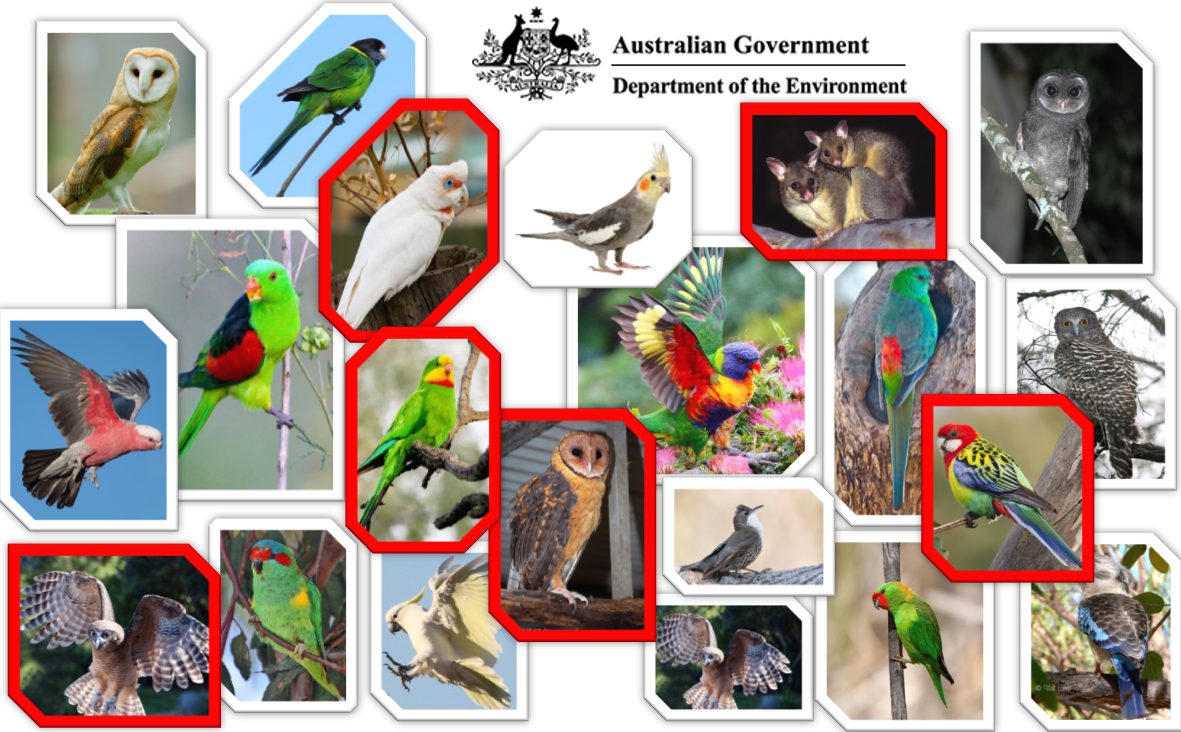
\includegraphics[width=\textwidth]{img/dead/Birds}
		\caption[Animals Closes to Exctinction]{A number of species that rely on tree hollows of which the red ones / bold ones are close to extinction: Kookaburra, Sulphur Crested Cockatoo, \textbf{Corella},  Crimson Rosella, Eastern Rosella,  Galah, Rainbow Lorikeet,  Musk Lorikeet, Little Lorikeet , Red-winged Parrot,  \textbf{Superb Parrot}, Cockatiel,   Australian Ringneck (Parrot),  Red-rumped Parrot,   Powerful Owl,    Sooty Ow,        Barking Owl, \textbf{Masked Owl},  \textbf{Barn Owl},  White-throated Treecreeper, Hollow Owl, \textbf{Brush-tailed Possum} (mammal) \footnotemark}
		\label{fig:Birds}
	\end{figure}
	\footnotetext{    	
		The images of the birds were taken from the following links (Retrieved on the 27th of April 2016):  
		Kookaburra: \url{<http://tenrandomfacts.com/blue-winged-kookaburra/>}, 
		Sulphur Crested Cockatoo: \url{<http://aussiegal7.deviantart.com/art/Sulphur-Crested-Cockatoo-08-153341893>},
		Corella: \url{<http://www.theparrotplace.co.nz/all-about-parrots/long-billed-corella/},     	Superb Parrot: \url{<http://www.davidkphotography.com/?showimage=637>},
		Crimson Rosella: \url{<http://25.media.tumblr.com/tumblr_m3mo89c40r1r4t9h1o1_1280.jpg>},
		Eastern Rosella: \url{<http://2.bp.blogspot.com/-pYxw51WjSOY/UB-LEFgd2KI/AAAAAAAAAWg/9z60PUWE6TE/s1600/_GJS6601-as-Smart-Object-1.jpg>},
		Rainbow Lorikeet: \url{<https://www.reddit.com/r/pics/comments/328fvc/a_rainbow_lorikeet_found_in_coastal_regions/>},     	Musk Lorikeet: \url{<http://www.rymich.com/girraween/photos/animals/birds/medium/glossopsitta_concinna/glossopsitta_concinna_001.jpg>},     	Little Lorikeet: \url{<http://www.pbase.com/sjmurray/psittacidae>},     	Red-winged Parrot: \url{<https://www.pinterest.com/pin/395894623469889727/>}, Cockatiel: \url{<http://up.parsipet.ir/uploads/Cockatiels-for-sale.jpg>},     	Australian Ringneck (Parrot): \url{<http://ontheroadmagazine.com.au/wp-content/uploads/2015/09/Twenty-eight-parrot-2-min.jpg>},     	Red-rumped Parrot: \url{<http://parrotfacts.net/wp-content/uploads/Red-Rumped-Parrot-on-a-tree.jpg>},     	Powerful Owl: \url{<http://farm1.staticflickr.com/219/495796536_f78dac04c1.jpg>},     	Sooty Owl: \url{<ttp://www.mariewinn.com/marieblog/uploaded_images/screech2-738532.jpg},     	Barking Owl: \url{<http://www.pcpimages.com/Nature-and-Wildlife/Birds/i-7JKSTp5/1/L/owl\%20\%281\%20of\%201\%29-L.jpg>},     	Masked Owl: \url{<http://www.survival.org.au/images/birds/masked_owl_2_600.jpg>},  	Galah: \url{https://www.pinterest.com/pin/537546905498955709/>},   	White-throated Treecreeper: \url{<https://geoffpark.files.wordpress.com/2011/09/female-white-throated-treecreeper.jpg>}, Hollow Owl: \url{<http://www.mariewinn.com/marieblog/uploaded_images/screech2-738532.jpg>} }
}





\subsection{Related Work}

\par Remote Sensing was introduced for automatically detecting dead trees, because fieldwork is time consuming considering their variance spread and the size of the relevant forests. From a classification perceptive, the task of identifying dead standing and dead fallen trees is different. Fallen trees are identified by detecting segments or line-like features on the terrain surface using LiDAR data \cite{Polewski2015} \cite{Mucke2013}. Regarding standing dead trees, their shape (reduced number of leaves or broken branches) \cite{Yao2012} and light reflectance (less green light illuminated) \cite{Pasher2009} are important factors for identifying them.


\par Previous work on dead standing trees detection performs single tree crown delineation before health assessment \cite{Yao2012} \cite{Shendryk2016_DeadTrees}. Tree-crown delineation is usually done by detecting local maxima from the canopy height model (CHM) and then segmenting trees with watershed algorithm \cite{Popescu2003}. Improvements has been achieved by introducing markers controlled watershed \cite{Jing2012} and structural elements of tree crowns with different sizes \cite{Hu2014}. Additionally, Popescu and Zhao analyse the vertical distribution of the LiDAR points in conjunction with the local maximum filtering of CHM \cite{Popescu2008}.


\par  In the case of Eucalyptus, single tree detection is a challenge on its own, due to their irregular structure and multiple trunk splits. In other words, each tree trunks splits create a local maximum leading into over-segmentation when tree crowns are detected by local maxima filtering. Shendryk published a eucalyptus delineation algorithm that starts segmentation from bottom to top. In this paper, the trunks point cloud is separated from the leaves and individual trunks are identified before proceeding to crown segmentation \cite{Shendryk2016_treeDeliniation}. Nevertheless, for that project only 17 flightlines of LiDAR data were collected. The density resolution starts from 12 points/$m^2$ and goes up to 36 points/$m^2$ around forested areas. For small research projects capturing this high resolution is acceptable, but for commercial use and larger areas, the density of data collected is above the optimal resolution for a cost effective versus quality acquisition \cite{Lovell2005}. The project of this thesis is much larger. The resolution of our acquired LiDAR data has an average of four pulses per square meter,{\color{blue} which is considered an optimal resolution in relation to the cost}. But because of the tree height (up to $43m$ according to the fieldwork), a small amount of pulse intensity reached the trunks and the recordered waveform do not include enough information for individual trunk detection.  An example of this project's discrete LiDAR data is shown in Figure \ref{fig:NoTrunks} and the missing information about the trunks is depicted.

\begin{figure} [h!]
	\centering
	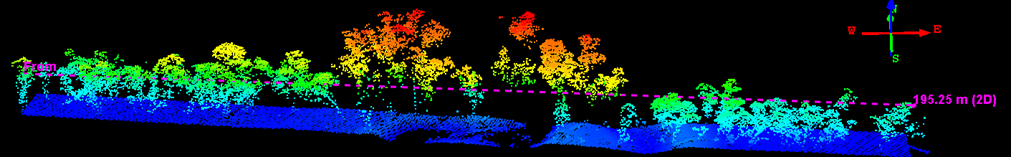
\includegraphics[trim={7cm 0 1.7cm 0},clip,width=\textwidth]{img/dead/TreesNoTrunks}
	\caption{LiDAR point cloud showing that there are very limited points reflected from tree trunks.}
	\label{fig:NoTrunks}
\end{figure}


{\color{red} ***Note read again to make sure it matches OK}
\par The acquired data are full-waveform LiDAR data. Traditional ways of interpreting FW LiDAR data, suggests extraction of a denser points cloud using Gaussian decomposition ~\cite{Neuenschwander2009} ~\cite{Reitberger2008}. Nevertheless, in this project we uses the open source software DASOS. DASOS was influenced by Persson et al, 2005, who used voxelisation to visualise the waveforms ~\cite{Persson2005}. But, it does not only uses voxelisation for visualisations but also for extracting metrics useful in classification. It further normalises the intensities so that equal pulse length exists inside each voxel, making intensities more meaningful. It is further seems that the literature is moving towards voxelisation with promising results obtained at recent publication on tree species classification ~\cite{Cao2016}. 

Here, it is introduced an approach for quick dead tree detection derived from the boost cascade approach \cite{Viola2001} but extended into 3D. This approach further contains similarities of the 3D tree shape signatures proposed by Dong, 2009, for distinguishing Oaks from Douglas fir tree crowns \cite{Dong2009}. 





%\subsection{Potentially add Objectives???}







\section{Materials}
% In this section, information about the study area, the acquired remote sensing and field data are provided. Figure \ref{fig:StudyArea} depicts all of them on a map, while section \ref{sec:StudyArea}, \ref{sec:AcquiredData} and \ref{sec:fieldData} give technical information about them. 

% {\color{red} *** NEIL: What information?} 

\subsection{Study Area} \label{sec:StudyArea}

The study area (Figure \ref{fig:StudyArea}) is a native River Red Gum (Eucalyptus camaldulensis) forest  of size $542km^2$ in south-eastern Australia. The regeneration of the eucalyptus is extremely dependant in floods and therefore, their distribution in respect to density, health and age is highly variance \cite{Kerle2005}. Additionally, the height of Eucalyptus camaldulensis reaches up to $30-40m$ and their structural complexity is high with multiple trunk splits \cite{Wilson1995}. The size and structure of the forest, with a human as reference, is depicted in Figure \ref{fig:EucalyptusSize}, while examples of the variance shape of dead trees is shown in Figure~\ref{fig:DeadTreesExamplePhotos}. 

\begin{figure} [h!]
	\centering
	\begin{framed}
		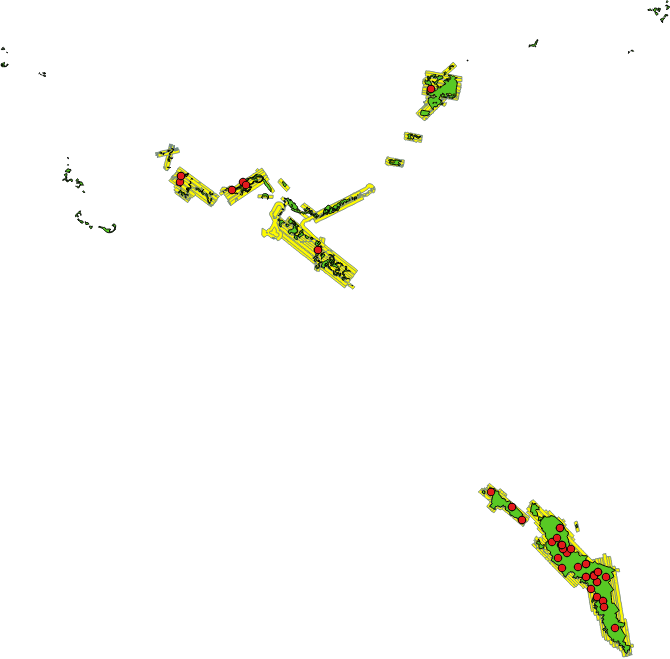
\includegraphics[width=0.965\textwidth]{img/dead/StudyArea}
	\end{framed}
	\caption{The study area is depicted by green ($542km^2$), the yellow strips are the LiDAR flightlines and the red dots are the position of the field plots.{\color{red}**Note: this image many need to be removed due to confidentiality of the company. I will talk with them and hopefully it will be ok.}}
	\label{fig:StudyArea}
\end{figure}

\begin{figure} [h!]
	\centering
	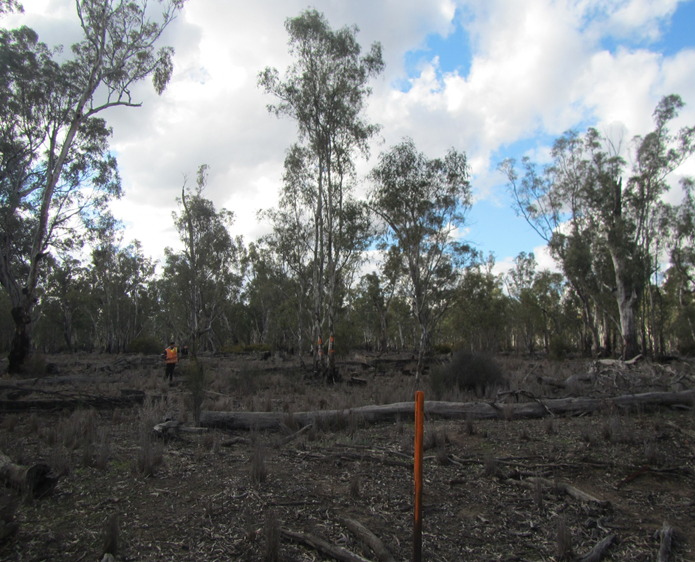
\includegraphics[width=0.965\textwidth]{img/dead/Eucalyptus.png}
	\caption{Structure of Red Gum Forest in south-eastern Australia.}
	\label{fig:EucalyptusSize}
\end{figure}

\begin{figure} [h!]
	\centering
	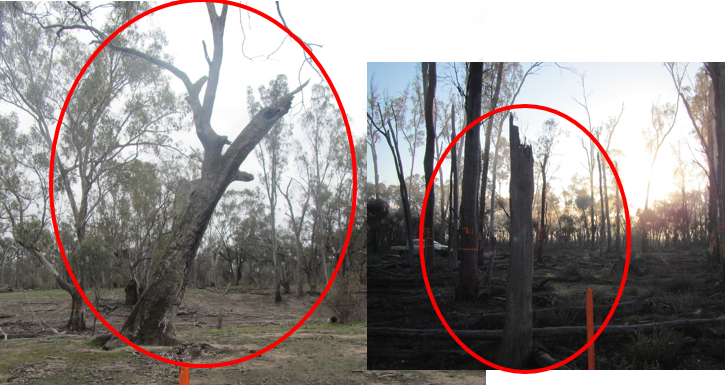
\includegraphics[width=0.965\textwidth]{img/dead/DeadTreesExamplePhotos}
	\caption{Example of dead trees indicating their variance in shape.}
	\label{fig:DeadTreesExamplePhotos}
\end{figure}

\subsection{Acquired full-waveform LiDAR data}\label{sec:AcquiredData}

\par Multiple-echo, full-waveform (FW) LiDAR data are supplied by RPS Australia East Pty Ltd. The data were acquired from 900m above ground level, using the Trimble AX60 Airborne LiDAR sensor, which was released in October 2013 \cite{Trimble}. The wavelength of the emitted laser was 1062nm, the maximum scan angle was 60 degrees, and the pulse rate was 400kHz. The acquisition was held from the 6th of March till the 31st of March 2015.  The collected LiDAR were delivered into 206 flightlines, of which 13 are cross runs used for geometric correction. There is also a 30\% of swath overlap. The point spacing along and across the track  is 0.48m and the average point spacing is 4.3 points per square meter. Figure \ref{fig:DeadTreeInLiDAR} shows an example of a dead tree in respect to the acquired discrete LiDAR point cloud.   Detailed information about FW LiDAR related concepts are given in section \ref{AcquireData}.



\begin{figure} [h!]
	\centering
	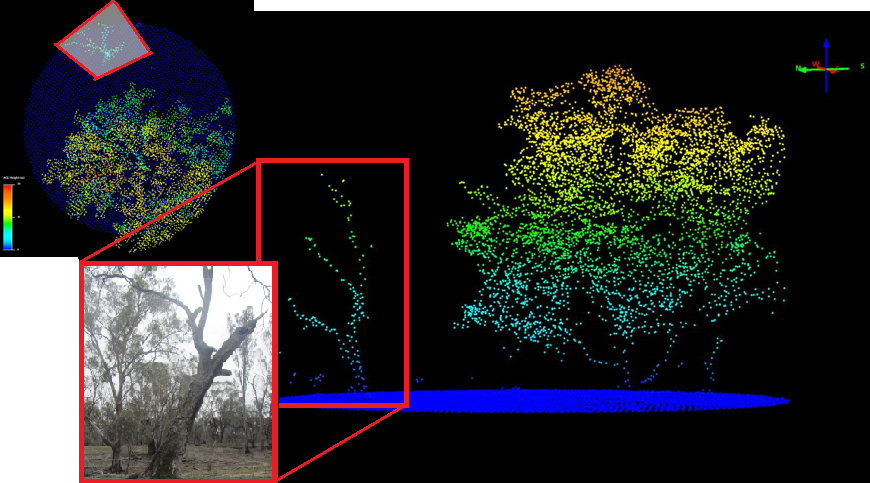
\includegraphics[width=\textwidth]{img/dead/DeadTreeInLiDAR}
	\caption{Example of a dead tree in relation to the discrete LiDAR point cloud.}
	\label{fig:DeadTreeInLiDAR}
\end{figure}



\subsection{Field Data}\label{sec:fieldData}

\par The field data were collected in July 2015 during the winter season of Australia and they include tree and canopy related measurements on circular plots. There are 33 plots with radius 35.68m and area 0.4ha  allocated randomly inside the study area. On these plots, a total of 2386 trees were individually measured.  Tree measurements include the geo-location, the trunk diameter at the standard height of 1.3m (breast heigh), height, species and health conditions (i.e. dead or alive). The geo-location of each tree is defined by the magnetic bearing from the centroid of the plot in degrees (range $[1,360]$) and the distance from the centroid in meters. The northing and easting coordinates of the geo-location of each tree were calculated in post-processing. Here is worth mentioning that a single tree may be recorded as multiple trees if there is a trunk split bellow the breast height of 1.3m. Furthermore, 91.59\% are River Red Gum and the rest are Black Box (Eucalyptus largiflorens) and Wattle group (Acacia spp.). 

\par Inside the field data, there are 260 dead trees recorded. Nevertheless, not all of those trees are considered useful for biodiversity. Dead trees with big Diameter at Breast Height (DBH) are more likely to contain hollows. Additionally, trees with DBH smaller than the footprint spacing of the LiDAR data are not identifiable from the FW LiDAR data. Table \ref{tab:DBH} shows the number of dead and alive trees in respect to their DBH. 

\begin{table}[!h]
	\centering
	\begin{tabular}{| l || c | c | }
		\hline		
		\textbf{DBH} &\textbf{Dead Trees} & \textbf{Alive Trees }\\	
		\hline			
		\hline			
		\textbf{>2000} & 0 & 1\\
		\hline			
		\textbf{1000-2000} & 7 & 21\\
		\hline			
		\textbf{600-1000} & 8 & 146\\
		\hline			
		\textbf{400-600} & 26 & 290\\
		\hline			
		\textbf{300-400} & 32 & 286\\
		\hline			
		\textbf{200-300} & 50 & 462\\
		\hline			
		\textbf{100-200} &125 & 904\\
		\hline			
		\textbf{<100} & 11 & 16\\
		\hline			
		\textbf{Total} & 260 & 2126 \\
		\hline  
	\end{tabular}
	\caption{Number of trees according to their DBH. {\color{red}**Note: I think it is in centimeter but I will confirm it with the company and add it afterwards. }}
	\label{tab:DBH}
\end{table}

\par Please note that the aforementioned field data were provided by Forestry Corporation of NSW, Wauchope, Australia and Interpine Ltd Group, New Zealand. For this thesis, a case study for collecting field data was conducted in New Forest, UK. This helped to better understand classification challenges in forestry applications. More information about this study is provided in Appendix \ref{Fieldwork}.

{\color{red} *** NEIL : everything from here is new ***}

\section{Challenges}
\par This section focuses on the challenges faced while working on the detection of dead standing eucalyptuses. Table \ref{tab:ClassificationChallenges} underlines the challenges, categorised into three groups: the nature of the study area, the acquired data and the field data. All these challenges influence the quality of the classifier and the accuracy of the results. 


\begin{table}[!h]
	\centering
	\begin{tabular}{| p{0.3\linewidth} ||  p{0.3\linewidth} ||  p{0.3\linewidth} | }
		\hline		
		\textbf{Study Area} &\textbf{Acquired Data} & \textbf{Field Data}\\	
		\hline			
		\hline
		\tabitem 	The study area is a native eucalyptus forest. Native forests contain trees of different ages and heights. The height of a dead tree could be within the range of [1.5,40] meters.\newline
		\tabitem The density of the forest is highly variance. Sometimes the testing/training priors of the small dead trees may contain information from either nearby alive trees or ground.  \newline 
		\tabitem A tree may have dead branches but still be alive. \newline
		\tabitem Eucalyptus trees have irregular shapes and multiple trunk splits making tree delineation to require very dense acquired data. 
		 &
		  \tabitem The pulse density of the acquired data does not allow bottom to top tree delineation. Crown detection from DEM (top) leads to over-segmentation due to the multiple trunk-splits. We, therefore, investigate the performance of object detection algorithms that do not require tree delineation.\newline
		  \tabitem An important factor of identifying dead trees is the light reflectance, but for this project this kind of data (i.e. coloured imagery) was acquired. Therefore, the classifier is only trained on tree shapes. But tree shape is not the only relevance, since a tree may not have leaves but still be alive.				 
		 & 
         \tabitem If a tree has a trunk split below the 1.3m height, then it is recorded as multiple trees within the field data. This confers inconsistency of the "one tree" concept.  \newline
		 \tabitem They contain small trees, which are non detectable from the acquired data. \newline
		 \tabitem The accuracy of the geo-spatial positions is unknown. Even though it is claimed to be in centimetres, there are trees clearing appearing on the ground once visualised on top of the DEM.
		  
		 \\
	
		\hline  
	\end{tabular}
	\caption{The Classification challenges of automated detection of dead eucalyptuses}
	\label{tab:ClassificationChallenges}
\end{table}

\section{Methods and Algorithms / Statistical Analysis}

\par steps

\begin{itemize}
	\item Subtract DTM From full-waveform LiDAR
	\item DASOS and 3D priors
	\item Random Forest for identifying the most significant features
	\item Nearest Neighbour 
	\item Thinning Algorithm
	\item Remove Ground and noisy columns using Gaussian decomposition
	\item Evaluation
\end{itemize}

\subsection{Subtract DTM from FW LiDAR}\label{sec:DTMsub}

\par DASOS has a feature for subracting pre-calculated Digital Terrain Model (DTM) saved into .bil files. Generating DTM is beyond the scope of this research and the DTM files used, were provided by Interpine Ltd Group. The provided DTM files were generated using the Quick Terrain Modeller from the discrete LiDAR using the parameters shown in Figure \ref{fig:DTM_parameters}.

\begin{figure} [h!]
	\centering
	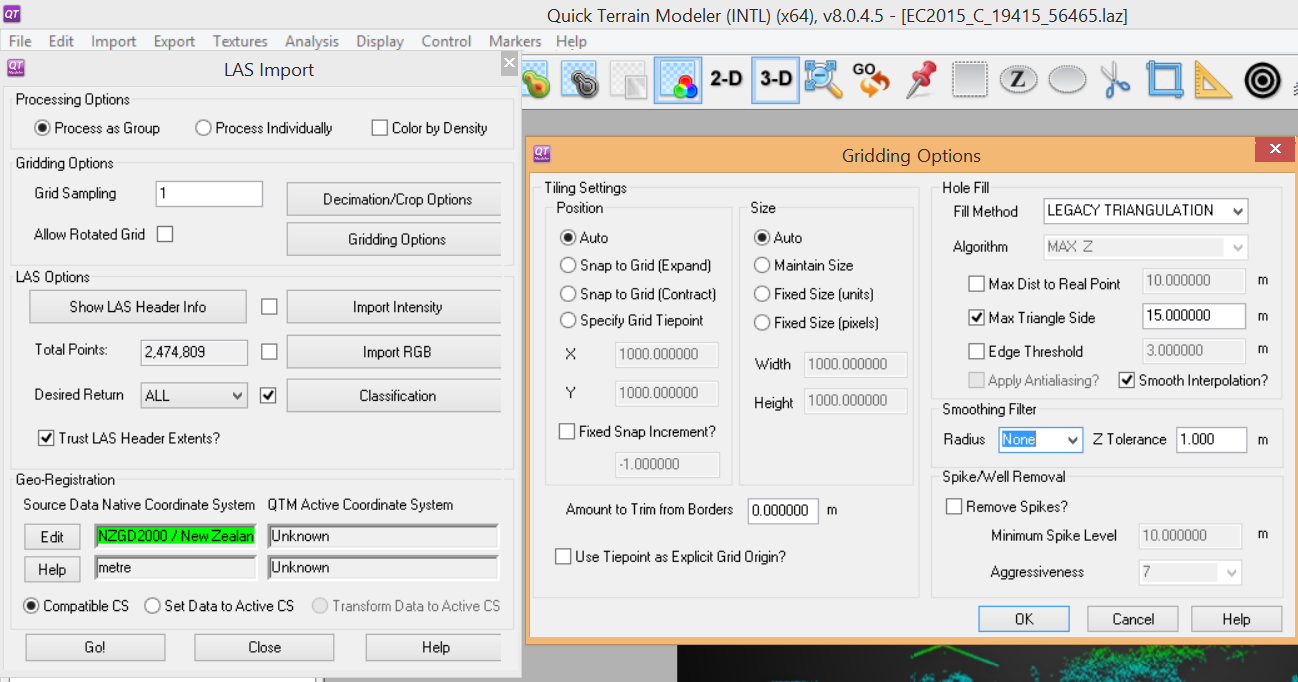
\includegraphics[width=\textwidth]{img/dead/DTM_parameters}
	\caption{Parameters used in Quick Terrain Modeller to obtain the DTM used here.}
	\label{fig:DTM_parameters}
\end{figure}


\par The subtraction of the DTM is done during the voxelisation (Section \ref{DASOS_Voxelisation}). The terrain height is subtracted from the position of the sample and then inserted into the volume. Please note that this terrain value is not subtracted from the origin of each pulse but from the position of each sample since the terrain value at the origin and the terrain value at the position of the sample may differ. Figure \ref{fig:height_minus_dtm} shows an example of a DEM generated before and after the subtraction using DASOS. 


\begin{figure} [h!]			
	\begin{subfigure}[t]{.49\textwidth}
		
		\centering
		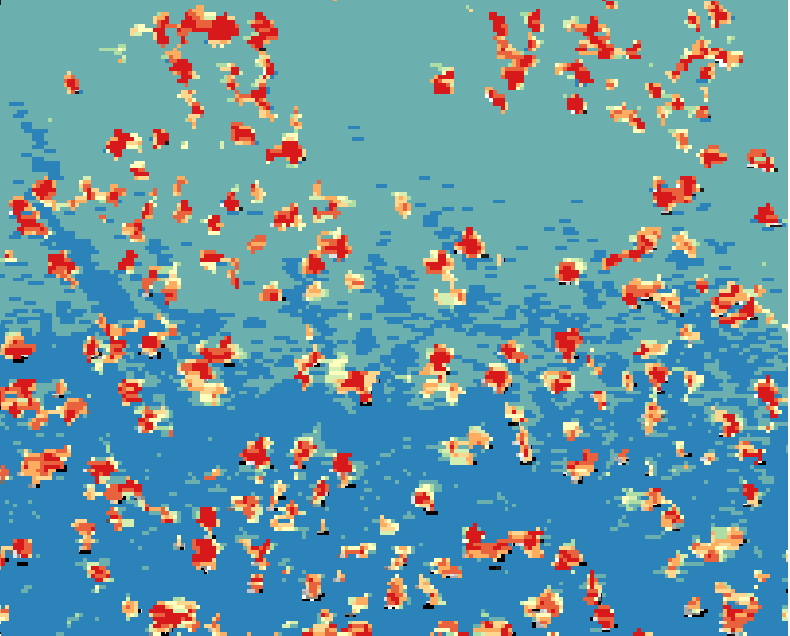
\includegraphics[width=\textwidth]{img/dead/height}
		\caption{The DEM before subtracting the DTM}
		\label{fig:height}
	\end{subfigure} \hfill
	\begin{subfigure}[t]{.49\textwidth}
		\centering
		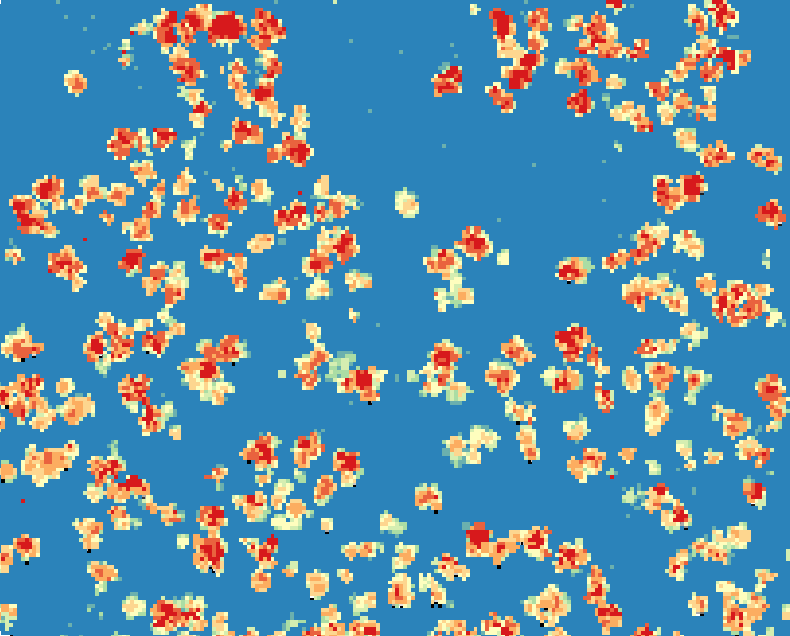
\includegraphics[width=\textwidth]{img/dead/height_dtm}
		\caption{The DEM after subtracting the DTM} 
		\label{fig:height_dtm}
	\end{subfigure} \hfill
	\caption{Showing the difference in the DEM before and after subtracting the terrain height. It is clearly shown that the ground in the right image is flat.}  
	\label{fig:height_minus_dtm} 
\end{figure}


\subsubsection{DASOS and 3D priors}

\par Here, the 3rd feature of DASOS (Table \ref{tbl:functionalities}) is used for generating 3D priors characterising dead standing Eucalypt trees.  This section explains how this feature works and what the training/testing data were obtained using this feature of DASOS. 

\par  In a few words, the 3D priors contain local information of small areas within the voxelised FW LiDAR space. 

The priors are exported into .csv files for easy manipulation into software packages for statistical analysis like R and matlab. For example, a 3D prior could contain information about a the shape of a dead tree. There are two options about the information exported and two options for the shape of the priors.  

The 3D shape signatures were generated by getting the distance distribution of random LiDAR point pairs of the two tree crown classes: Oaks and Douglas \cite{Dong2009}







\par Figure \ref{fig:DASOSsPriors}


\begin{figure} [h!]
	\centering
	\includegraphics[width=\textwidth]{img/dead/DASOSsPriors}
	\caption{This figure shows what priors were created for testing and how they are divided for cross validation.}
	\label{fig:DASOSsPriors}
\end{figure}



\par By the end it is worth mentioning that the dead tree detection is the first application of the 3D priors feature of DASOS, which was released on the 20th of January 2017 \cite{DASOS_v2}. 

\newpage
	\begin{longtable}
		{|p{4.65cm}|p{9.45cm}|}
		\toprule
		\multicolumn{2}{|c|}{\textbf{Explanation of the 3D priors Output with the Processed Intensities}} \\
		\midrule
		\textbf{Label} & \textbf{Description} \\ 
		\cmidrule(r){1-1}\cmidrule(l){2-2}
		Height\_Middle\_Column& The height of the middle column of the prior
		\\
		\cmidrule(r){1-1}\cmidrule(l){2-2}
		Height\_Mean& The Mean height of all the columns included in the template\\
		\cmidrule(r){1-1}\cmidrule(l){2-2}
		Height\_Median& The Median height of all the columns included in the template
		\\
		\cmidrule(r){1-1}\cmidrule(l){2-2}
		Height\_Std&The Standard Deviation of the heights of the columns included in the template \\
		\cmidrule(r){1-1}\cmidrule(l){2-2}
		Sum\_Int\_Diff\_X& The Mirror Summed Difference of the intensities using the middle column in the x-axis as the axis of symmetry \\
		\cmidrule(r){1-1}\cmidrule(l){2-2}
		Sum\_Int\_Diff\_Y& The Mirror Summed Difference of the intensities using the middle column in the y-axis as the axis of symmetry\\
		\cmidrule(r){1-1}\cmidrule(l){2-2}
		Sum\_Int\_Diff\_Z& The Mirror Summed Difference of the intensities using the middle column in the z-axis as the axis of symmetry\\
		\cmidrule(r){1-1}\cmidrule(l){2-2}
		Max\_Int& The maximum intensity found inside the prior\\
		\cmidrule(r){1-1}\cmidrule(l){2-2}
		Min\_Int& The minimum intensity found inside the prior\\
		\cmidrule(r){1-1}\cmidrule(l){2-2}
		Ave\_Int& The average intensity of the voxels that contain an intensity above the isolevel\\
		\cmidrule(r){1-1}\cmidrule(l){2-2}
		Median\_Int& The median intensity of the voxels\\
		\cmidrule(r){1-1}\cmidrule(l){2-2}
		Per\_Int\_Above\_Iso& Percentage of voxels that contain an intensity above the isolevel\\
		\cmidrule(r){1-1}\cmidrule(l){2-2}
		Dis\_Mean& Mean distance from the central voxel to every voxel that contain san intensity above the isolevel  \\
		\cmidrule(r){1-1}\cmidrule(l){2-2}
		Dis\_Median& Median distance from the central voxel to every voxel that contains an intensity above the isolevel \\
		\cmidrule(r){1-1}\cmidrule(l){2-2}
		Dis\_Std& The Standard Deviation of the distances between the central voxel and every voxel that contains an intensity above the isolevel\\
		\cmidrule(r){1-1}\cmidrule(l){2-2}
		Top\_Patch\_Len\_Middle\_Col& The length of the top patch of the middle column of the prior\\
		\cmidrule(r){1-1}\cmidrule(l){2-2}
		Top\_Patch\_Len\_Mean& The Mean length of all the top patches\\
		\cmidrule(r){1-1}\cmidrule(l){2-2}
		Top\_Patch\_Len\_Median& The Median length of all the top patches \\
		\cmidrule(r){1-1}\cmidrule(l){2-2}
		Top\_Patch\_Len\_Std& The Standard Deviation of all the top patches \\
		\cmidrule(r){1-1}\cmidrule(l){2-2}
		Mirror\_Diff\_X\_Mean& The Mean Mirror Difference of the voxel intensities with the middle column of the x-axis as the symmetric axis\\
		\cmidrule(r){1-1}\cmidrule(l){2-2}
		Mirror\_Diff\_X\_Median& The Median Mirror Difference of the voxel intensities with the middle column of the x-axis as the symmetric axis \\
		\cmidrule(r){1-1}\cmidrule(l){2-2}
		Mirror\_Diff\_X\_Std& The Standard Deviation Mirror Difference of the voxel intensities with the middle column of the x-axis as the symmetric axis \\
		\cmidrule(r){1-1}\cmidrule(l){2-2}
		Mirror\_Diff\_Y\_Mean&  The Mean Mirror Difference of the voxel intensities with the middle column of the y-axis as the symmetric axis \\
		\cmidrule(r){1-1}\cmidrule(l){2-2}
		Mirror\_Diff\_Y\_Median&The Median Mirror Difference of the voxel intensities with the middle column of the y-axis as the symmetric axis 
		\\
		\cmidrule(r){1-1}\cmidrule(l){2-2}
		Mirror\_Diff\_Y\_Std& The Standard Deviation Mirror Difference of the voxel intensities with the middle column of the y-axis as the symmetric axis\\
		\cmidrule(r){1-1}\cmidrule(l){2-2}
		Mirror\_Diff\_Z\_Mean&The Mean Mirror Difference of the voxel intensities with the middle column of the z-axis as the symmetric axis \\
		\cmidrule(r){1-1}\cmidrule(l){2-2}
		Mirror\_Diff\_Z\_Median& The Median Mirror Difference of the voxel intensities with the middle column of the z-axis as the symmetric axis \\
		\cmidrule(r){1-1}\cmidrule(l){2-2}
		Mirror\_Diff\_Z\_Std& The Standard Deviation of the Mirror Difference of the voxel intensities with the middle column of the z-axis as the symmetric axis \\
		\bottomrule
		\caption[DASOS's functionalities]{The three functionalities of DASOS}
		\label{tbl:PriorsOutExplanation}	
	\end{longtable}

	\par In the following section, the images and examples are taken from the Cylinder processed parameters but it done for all four test cases and cross validated using the 5 datasets division.




\subsection{Random Forest}
	\par Images and examples for Cylinder processed parameters but it done for all four test cases and cross validated using the 5 datasets division.
	
	
	\par Random Forest failed to find relation between the 3D priors with the Raw Intensities due to the irregular shapes of Eucalyptus trees and probably due to the scan from different angles. Raw Intensities may be useful for identifying pine trees in commercial forest, where the variance between each other is smaller. 

	
	\par Therefore from here we only test processed intensities with 3D cylindrical and 3D  rectangular cuboid priors. 
	
	\par Identified the most significant features for detecting dead trees and then we build the following probabilistic model. 
	
	
	\begin{figure} [h!]			
		\begin{subfigure}[t]{.49\textwidth}
			
			\centering
			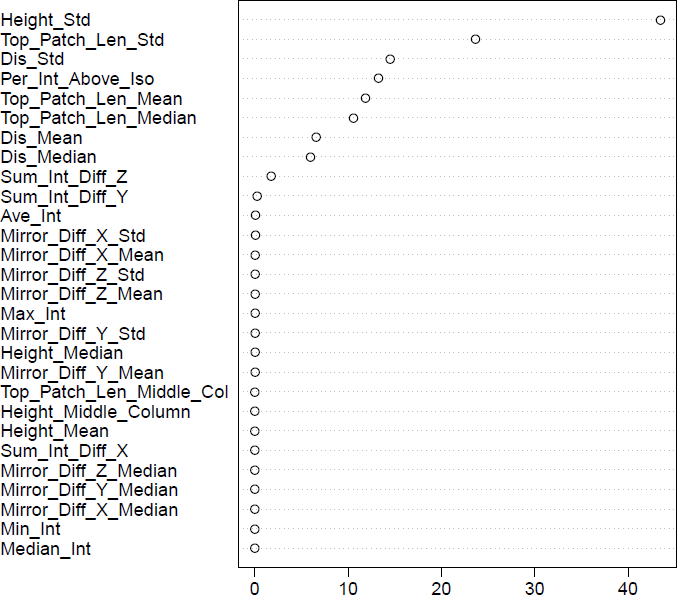
\includegraphics[width=\textwidth]{img/dead/c0_random_forest}
			\caption{.}
			\label{fig:c0_RandomForest}
		\end{subfigure} \hfill
		\begin{subfigure}[t]{.49\textwidth}
			\centering
			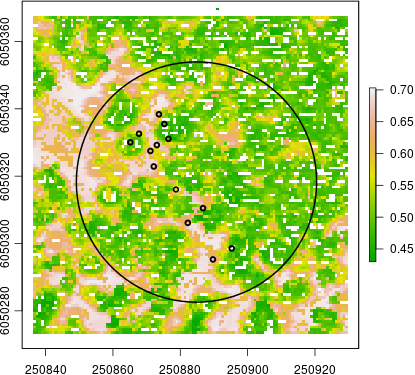
\includegraphics[width=\textwidth]{img/dead/c1_knn}
			\caption{.} 
			\label{fig:c1_knn}
		\end{subfigure} \hfill
		\begin{subfigure}[t]{.49\textwidth}
			\centering
			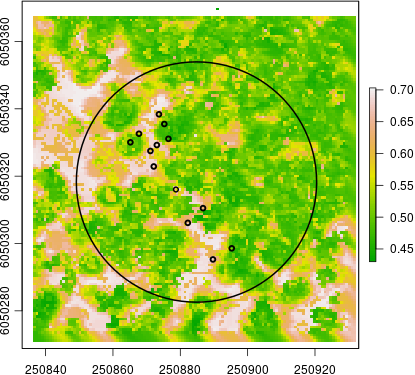
\includegraphics[width=\textwidth]{img/dead/c2_knn_SaltPepper}
			\caption{} 
			\label{fig:c2_SaltPepper}
		\end{subfigure}
		\begin{subfigure}[t]{.49\textwidth}
			\centering
			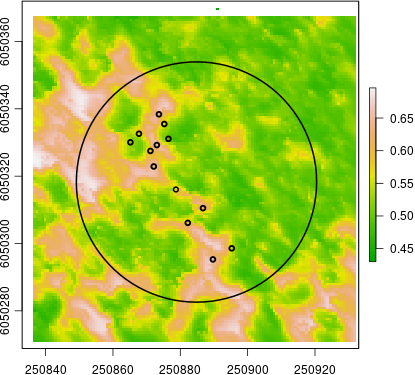
\includegraphics[width=\textwidth]{img/dead/c3_knn_smoothed}
			\caption{} 
			\label{fig:c3_Smoothed}
		\end{subfigure}
		\caption{ }  
		\label{fig:RF_knn_salt_smooth} 
	\end{figure}
	
	
	
\subsection{Probabilistic Model}

\par We don't go straight to classification because in the testing data, we put a prior for each column and therefore many columns that contain dead trees are not marked correctly. And we wrote a probabilistic model using the most significant features identified by the random forest. 

 \par k-nearest neighbour: distance from the centre of mean for each of the first 5 significant features 
 \par P = P(dead)/(P(dead)+P(alive)) 
 \par from that get grey scale field of the results 



 
 

 
 
 \subsection{Ground Mask}
 \par threshold ground: Histogram of heights, because subtracted DTM,everything below 20 is considered ground. 
 \par Great histogram of the height map generated using the 2D metrics of DASOS. 
 
 \par Create three classes : ground, trees and noise
 
 \par Because the DTM has been subtracted (Section \ref{sec:DTMsub}), the ground is easily separated from the trees. 
 
 \par Mask out  ground and noise
 \begin{figure} [h!]			
 	\begin{subfigure}[t]{.49\textwidth}
 		
 		\centering
 		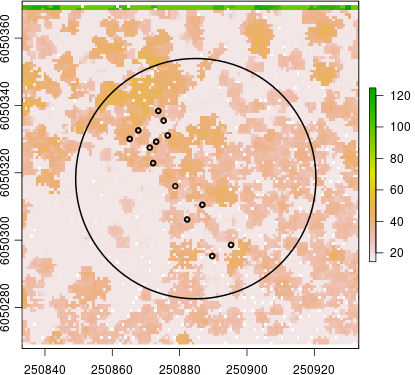
\includegraphics[width=\textwidth]{img/dead/c4_height}
 		\caption{.}
 		\label{fig:c4_height}
 	\end{subfigure} \hfill
 	\begin{subfigure}[t]{.49\textwidth}
 		\centering
 		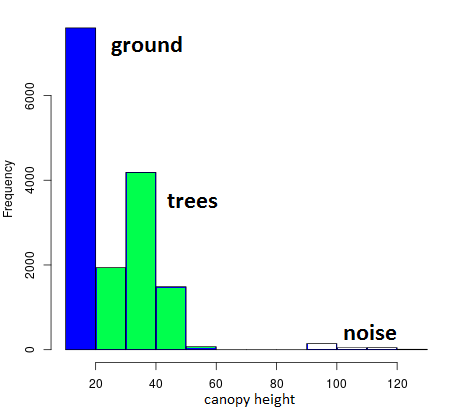
\includegraphics[width=\textwidth]{img/dead/c5_histHeight}
 		\caption{.} 
 		\label{fig:c5_heightHist}
 	\end{subfigure} \hfill
 	\begin{subfigure}[t]{.49\textwidth}
 		\centering
 		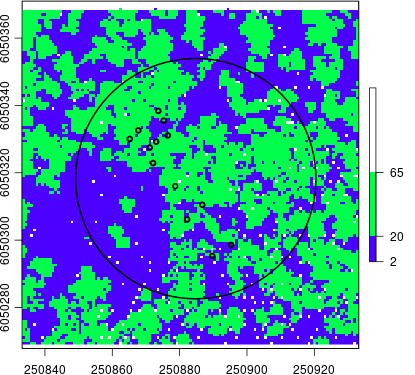
\includegraphics[width=\textwidth]{img/dead/c6_groundThres}
 		\caption{} 
 		\label{fig:c6_groundMask}
 	\end{subfigure}
 	\begin{subfigure}[t]{.49\textwidth}
 		\centering
 		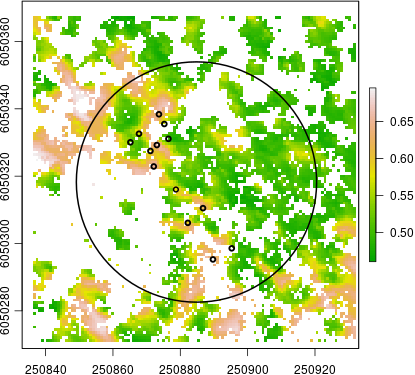
\includegraphics[width=\textwidth]{img/dead/c7_groundRemoved}
 		\caption{} 
 		\label{fig:c7_groundRemoved}
 	\end{subfigure}
 	\caption{ }  
 	\label{fig:GroundPixelsRemoval} 
 \end{figure}
 
 
 \subsection{Filtering and Local Maxima}
 \par Salt and pepper filter
 \par Smoothing filter 
 

 

 
 
 \subsection{Threshold}
  \begin{figure} [h!]			
  	\begin{subfigure}[t]{.49\textwidth}
  		
  		\centering
  		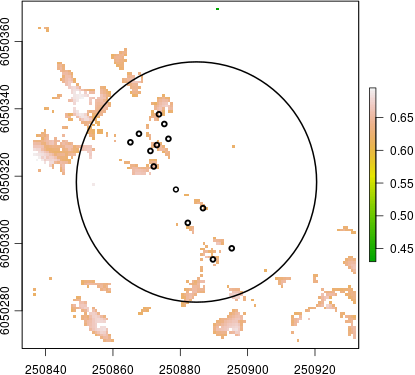
\includegraphics[width=\textwidth]{img/dead/c8_thresDead}
  		\caption{.}
  		\label{fig:c8_deadThres}
  	\end{subfigure} \hfill
  	\begin{subfigure}[t]{.49\textwidth}
  		\centering
  		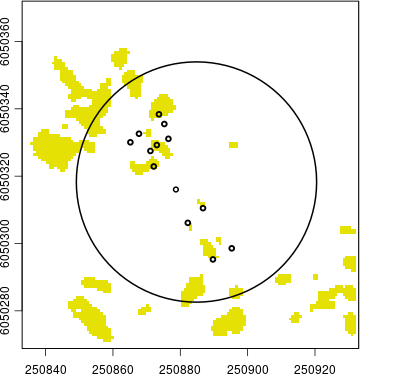
\includegraphics[width=\textwidth]{img/dead/c9_sharpFilter}
  		\caption{.} 
  		\label{fig:c9_sharpFilter}
  	\end{subfigure} \hfill
  	\begin{subfigure}[t]{.49\textwidth}
  		\centering
  		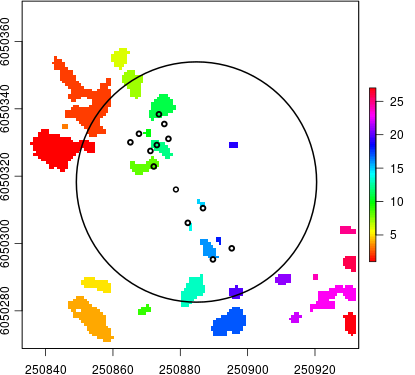
\includegraphics[width=\textwidth]{img/dead/c10_segmentationResults}
  		\caption{} 
  		\label{fig:c10_segmentation}
  	\end{subfigure}
  	\begin{subfigure}[t]{.49\textwidth}
  		\centering
  		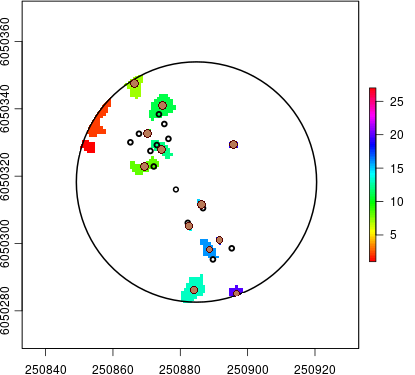
\includegraphics[width=\textwidth]{img/dead/c11_TreePos}
  		\caption{} 
  		\label{fig:c11_results}
  	\end{subfigure}
  	\caption{ }  
  	\label{fig:dt_sf_segm_results} 
  \end{figure}
  
 \par if a local maxima is found but the probability of being a dead is low then it is not a dead tree. This is defined by a user defined constant threshold. 
 
  \par threshold values according to the probability of been a dead tree >0.62
 
 \subsection{Segmentation}
  \par remove pixels that have <3 neighbouring dead pixels and add those which have plenty around them
  \par seed point growth segmentation algorithm
  
  \subsection{Assign dead tree position}
  \par for each segment find the middle pixel and assign that as a dead tree


\newpage
\section{Evaluation} 

   \subsection{Distance Related Evaluation}


   \subsection{Pixelwise Evaluation}
		
		
\section{Discussion}

\par Dead tree detection is a difficult task due to the irregular shapes of the trees and different sizes. Here we produced this algorithm (pla pla) which is new because it doesn't need tree segmentation but has a lot of room for improvement. 

Also don't know the accuracy of the tree position and as we can see at some heigh maps there are places where there are trees according to the fieldplots but the data clearly shown that there are not trees
\section{Future Work}

\begin{itemize}
	\item Manually check and improve position of dead trees using visualisations of the data. In order to improve accuracy of test and evaluating data
	\item Separate trees from field data according to their height because tree with different heights have different shape properties and the priors used had constant size
	\item Create priors that have adjustable size according to the height of the tree	
	\item After the seed growth algorithm, check the size of the segments and look into the possibility of merging two segments into one or dividing a segments into multiple sub-segments.
	\item Test the results when only using dead trees for training data and not alive
	\item The system is usually confused at the edges of the alive trees. Research on how this could be improved. 
\end{itemize}

\end{document}